\chapter{State of the Art}\label{section:stateoftheart}

\section{Introduction}
This chapter provides an overview of the current state of smart irrigation 
systems and their applications in agriculture. 
This chapter will explore the existing technologies, methods, and solutions used in smart irrigation. 
It will also highlight the gaps and challenges in the current systems,
and how the PiIrrigate project tries to address these issues.

\section{Existing Smart Irrigation Solutions}
\subsection{Types of Smart Irrigation Systems}
\begin{itemize}
  \item \textbf{Weather-Based Controllers} \\
  This type of systems will use data collected from weather stations to optimize the irrigation schedules.
  Collected data consists of temperature, humidity and rainfall forecasts. Weather based controllers are not
  very precise as it does not use data from the soil, but it may be good enough for some use-cases.

  \item \textbf{Soil Moisture-Based Controllers} \\
  Soil moisture based controllers use sensors that are placed in the soil to measure
  the moisture level and adjust the irrigation accordingly.
  These are more precise than weather-based controllers, as they take into account
  the actual moisture level in the soil, but they require more maintenance and calibraiton
  \cite{smartIrrigationTechnologyControllersAndSensors}.

  \item \textbf{Hybrid Systems} \\
  Many modern systems utilize a hybrid approach, combining data from both
  weather feeds and soil moisture sensors for more accurate and resilient 
  irrigation decisions. Some research also explores "hybrid" in terms of 
  integrating different energy sources (e.g., solar and wind) to power the systems or 
  combining various 
  irrigation methods (like drip and sprinkler) under one smart control\cite{soilBasedIrrigation}.

  The PiIrrigate project place itself in the category of hybrid systems, using both
  soil moisture sensors and weather sensors to collect data.
  
  Some of the most popular hybrid smart irrigation systems include:
  \begin{itemize}
    \item \textbf{Netafim's Precision Irrigation System} \\
    This system cobines data from soil moisture and flow sensors with sattelite weather data and predictive
    analytics to optimize the irrigation proccess.
    
    Key features include:
    \begin{itemize}
      \item Real-time monitoring of soil moisture levels and weather forecasts.
      \item Automated irrigation scheduling based on weather forecasts.
      \item AI-based algorithms to optimize the irrigation timing and duration.
    \end{itemize}

    \item \textbf{CropX Smart Farming System} \\
    CropX is a cloud based platform that integrates soil moisture sensors, weather data and
    machine learning algorithms to optimize the irrigation process.

    Key features include:
    \begin{itemize}
      \item Irrigation recomandations based on soil variability, crop type and weather.
      \item Farmers can apply recommandations or integrate with automated irrigaitons contrllers.
      \item Easy to scale and adapt to different farm sizes from small to large-scale farms.
    \end{itemize}
  
    \item \textbf{Toro EVOLUTION® Series Controller with Smart ET Sensor} \\
    Combines basic sprinkler system hardware with smart sensors and connectivity,
    offering both manual and intelligent irrigation options. The evaporation sensors are used to measure
    the amount of water lost throught evaporation and adjust the irrigation accordingly.

    Key features include:
    \begin{itemize}
      \item Can be programmed manually or connected to a local weather station.
      \item Smart ET sensor measures evaporation rates and adjusts irrigation schedules.
      \item Compatible with smart devices for remote monitoring
    \end{itemize}
  \end{itemize}
\end{itemize}

\section{Comparative Analysis of Smart Irrigation Systems}
The table below provides a comparative analysis of some of the most popular smart 
irrigation systems available today and the PiIrrigate system.

\begin{table}[ht]
\centering
\begin{tabular}{|p{3.2cm}|p{3.2cm}|p{3.2cm}|p{3.2cm}|p{3.2cm}|}
\hline
\textbf{Feature} & \textbf{Netafim} & \textbf{CropX} & \textbf{Toro ET} & \textbf{PiIrrigate} \\
\hline
Irrigation Type & Drip & Any & Sprinkler & Custom \\
\hline
Automation & High (AI) & Med–High & Medium & Medium \\
\hline
Sensors & Soil, flow, weather & Soil, temp & ET sensor & Soil, temp, rain \\
\hline
Weather Data & Yes & Yes & Yes & Optional \\
\hline
Manual Control & App/cloud & App/web & Panel/app & Web UI \\
\hline
AI/Analytics & Yes & Yes & No & No \\
\hline
Scalability & Large farms & Small–large & Residential & Small farms/gardens \\
\hline
Cloud Sync & Yes & Yes & Optional & Yes \\
\hline
Use Case & Precision agri & Smart farming & Lawn care & Small to large scale\\
\hline
Cost & High & Med–High & Low–Mid & Low \\
\hline
\end{tabular}
\caption{Comparison of Smart Irrigation Systems}
\label{tab:irrigation_comparison}
\end{table}

\section{IoT and LoRa in Agriculture}
Agriculture is one of the biggest industries, critical to the global economy and food security. With the increasing food 
demant, the need for efficient and sustainable agricultural has grown in the last years. The IoT (Internet of Things) is
is a key technology that can help to address these challenges by providing real-time data and 
insights into the agricultural processes. LoRa (Long Range) is a wireless communication technology 
that is well suited for agriculture applications. It has been inmvented in 2009 \- 2010 by the company Cycleo, 
which was later acquired by Semtech in 2012 and until 2020 it was implemented in more than 100 million devices worldwide
\cite{LoRaHistory}.

One approach to integrate IoT and LoRa in agriculture it's to use a layered architecture.
This architecture consists of four layers: data aquisition, gateways, network and application.
where the sensors and actuators are connected to a LoRa gateway, which is then connected to a cloud platform. 
This architecture is proposed in this paper \cite{loraBasedIoTPlatform} and it is a similar approach to the one used in the 
PiIrrigate project. The sensors collect data from the environment, such as soil moisture, temperature, and humidity,
and send it to the LoRa gateway using LoRa radio communication. The gateway then sends the data to a cloud platform, 
where it can be processed and analyzed. The cloud platform can also send commands to the actuators, such as irrigation valves, 
to control the irrigation process based on the data collected by the sensors. 

\begin{figure}[H]
    \centering
    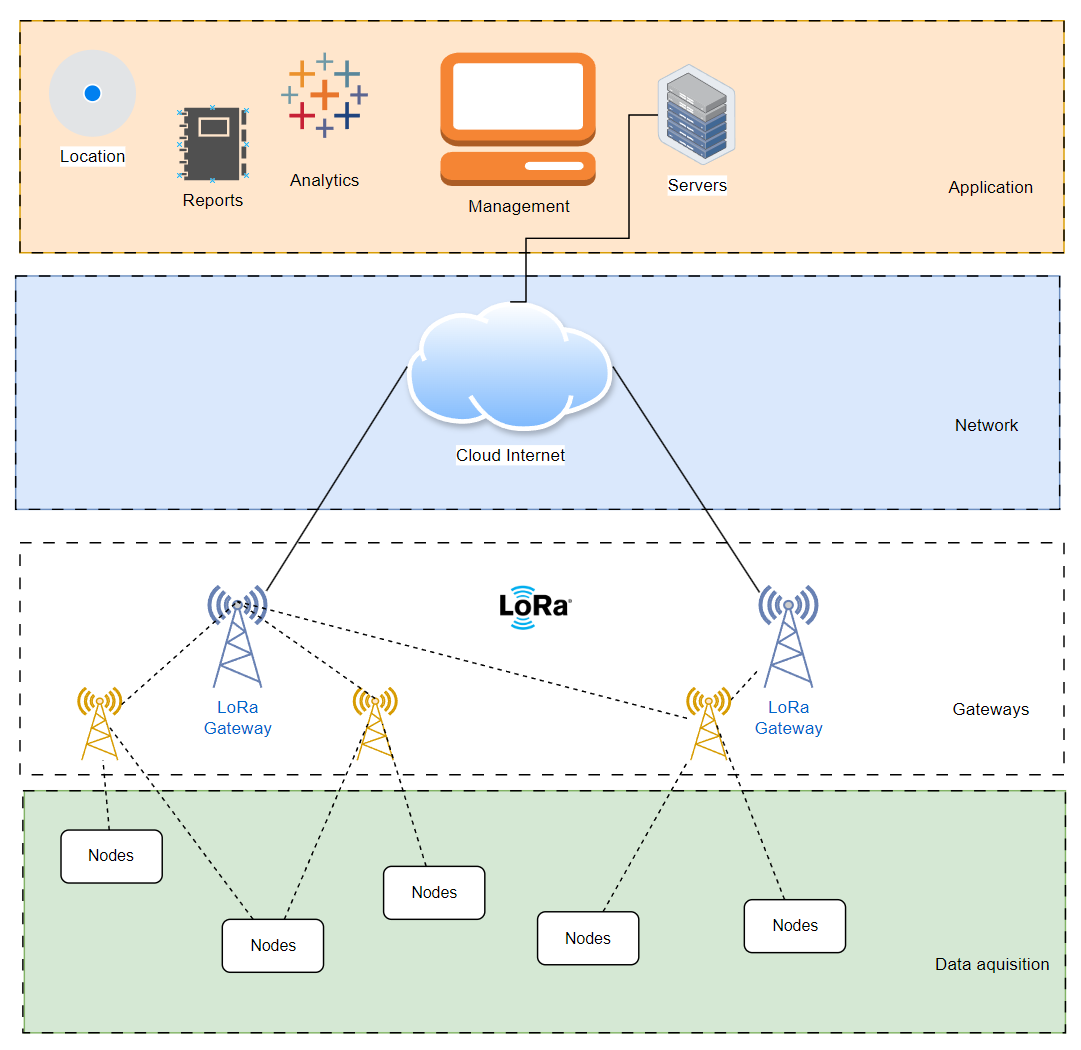
\includegraphics[width=0.7\textwidth]{images/loraWan.png}
    \caption{LoRa-based IoT Architecture for Agriculture}
    \label{fig:lora_architecture}
\end{figure}

\section{LoRa vs Other Wireless Technologies}
At this moment, theere are several wireless technologies available for IoT applications. After a 
comparative analysis of the most popular wireless technologies used in IoT, LoRa came out as one of the most suitable
technologies for smart irrigation systems because of its long range, low power consumption and scalability.
The table below compares LoRa with other wireless technologies commonly used in IoT applications, such as Wi-Fi, Bluetooth (BLE), 
Zigbee, and NB-IoT. In this section We will analyze the capabilities of these technologies
and their suitability for smart irrigation systems. The comparison is based on several features, 
including range, data rate, power consumption, topology, license band, scalability, cloud integration, infrastructure cost and latency.

Wifi, Bluetooth and Zigbee have a decent data rate, and very good latency, but they have a very short range 
and high power consumption. This makes them more suitable for local applications, 
such as home automation or local sensor networks. 
NB-IoT(Narrowband IoT) represents a poteantial solution for smart irrigation systems, but 
it has a higher infrastructure cost and requires a cellular network, which may not be available in all areas.

\begin{table}[ht]
\centering
\begin{tabular}{|p{3.2cm}|p{2.6cm}|p{2.6cm}|p{2.6cm}|p{2.6cm}|p{2.6cm}|}
\hline
\textbf{Feature} & \textbf{LoRa} & \textbf{Wi-Fi} & \textbf{Bluetooth (BLE)} & \textbf{Zigbee} & \textbf{NB-IoT} \\
\hline
Range & 2–15 km & $\sim$100 m & 10–100 m & 10–100 m & 10–35 km \\
\hline
Data Rate & 0.3–50 kbps & Up to 600 Mbps & Up to 2 Mbps & 20–250 kbps & Up to 250 kbps \\
\hline
Power Consumption & Very Low & High & Very Low & Low & Low \\
\hline
Topology & Star (LoRaWAN) & Star & Star & Mesh & Star (cellular) \\
\hline
License Band & Unlicensed (ISM) & Unlicensed (2.4 GHz) & Unlicensed (2.4 GHz) & Unlicensed (2.4 GHz) & Licensed \\
\hline
Scalability & High & Low & Low–Medium & Medium & High \\
\hline
Cloud Integration & Easy via LoRaWAN & Native IP stack & Requires gateway & Requires gateway & Native via operator \\
\hline
Infrastructure Cost & Low & Medium & Low & Medium & High \\
\hline
Latency & High (seconds) & Low (ms) & Very Low (ms) & Low (ms) & Moderate \\
\hline
Ideal Use Case & Smart City Infrastructure & Local, high-speed data transfer & Short-range sensors/wearables & Indoor sensor networks & National-scale deployment \\
\hline
\end{tabular}
\caption{Comparison of Wireless Technologies for Smart Irrigation}
\label{tab:wireless_comparison}
\end{table}


\section{Identified Gaps and Challenges}
Despite the advancements in smart irrigation systems, several gaps and challenges remain:

\begin{itemize}
  \item \textbf{High Costs} \\
  Many existing systems are expensive, making them inaccessible for small farmers or home gardeners.
  
  \item \textbf{Complexity of Use} \\
  Some systems require specialized knowledge to set up and maintain, which can be a barrier for adoption.

  \item \textbf{Limited Customization} \\
  Many commercial solution are designed for speicific crops and environments and that limits their
  applicability to diverse agricultural settings.
  \item \textbf{Data Integration Issues} \\
  Integration of data from different sources (e.g. wather, soil) can be more 
  complex and it can lead to inefficiencies in the irrigaiton management.
\end{itemize}

In addition to the gaps mentioned, there are a few other issues that must be resolved, 
like the need for systems that can function in challenging environmental conditions, 
the need for dependable internet connectivity in remote locations, and data security and privacy issues. 

The effect that smart irrigation systems have on the environment is another factor that must be 
taken into account.
Even though these systems are made to use water as efficiently as possible, the manufacturing 
and disposal of electronic components can harm the environment.
Therefore, developing sustainable and ecologically friendly systems is another challenge. 
This means that the systems should be built to last a long time and be simple to use, 
and that the parts used in them should be composed of recyclable materials.

\section{Summary}
In summary, the state of the art in smart irrigation systems shows significant 
advancements in technology and methods, but also highlights several gaps and challenges 
that need to be addressed. The PiIrrigate project aims to fill these gaps by providing a
cost-effective, easy-to-use, and customizable solution that leverages the power of IoT and LoRa 